\subsection{Parámetros de la ecuación de estado cúbica}

\begin{equation}
	b_i = \Omega_b \frac{R T_{ci}}{p_{ci}} 
\end{equation}

\begin{equation}
 a_i = \Omega_a \frac{\left(R T_{ci}\right)^2}{p_{ci}} \alpha_i
\end{equation}

En las secciones anteriores se usaron los parámetros a y b de la eq. de estado cúbica para el heptano. 

Estos parámetros dependen de la eq. de estado cúbica, expresión de \alpha y si la ecuación es utilizada para representar a una mezcla también dependen de la regla de mezclado.

La expresión de $\alpha$ puede ser una función de la temperatura





\begin{figure}[!h]
  
  \centering
    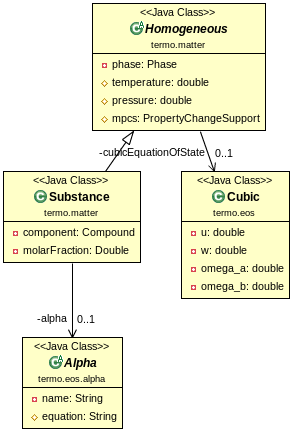
\includegraphics[scale=0.7]{cubic.png}
    \caption{A picture of a gull.}
\end{figure}


